% !TEX program = pdflatex
\documentclass[11pt]{article}

\usepackage[T1]{fontenc}
\usepackage[utf8]{inputenc}
\usepackage[margin=1in]{geometry}
\usepackage{amsmath,amssymb,amsthm}
\usepackage{graphicx}
\usepackage[authoryear,round]{natbib}
\usepackage[hidelinks]{hyperref}

\graphicspath{{../figures/}}

\theoremstyle{plain}
\newtheorem{lemma}{Lemma}
\newtheorem{proposition}{Proposition}
\newtheorem{corollary}{Corollary}
\theoremstyle{definition}
\newtheorem{assumption}{Assumption}

\title{Market Integration, Platformization, and Local Multipliers:\\
The Spatial Reorganization of Value Capture}
\author{Wenxiao Dong \and Yaqi Hu}
\date{\today}

\begin{document}

\maketitle

\begin{abstract}
Using a standard local-income multiplier closure, we study how integration
reallocates regional expenditure across channels with local
retention. We let capacity raise platform retention without changing prices or
demand. With no outside-funded retail spending, an endpoint-crossing condition
yields ordered thresholds: both nominal and consumption-equivalent real income fall
at low capacity, only the latter rises at intermediate capacity, and both rise
at high capacity. When platform retention is below local-agent retention, any
homothetic two-channel demand system with a strictly concave share-speed
generates a unique capture-drag peak, located below one-half under symmetry.
Integration and capacity have increasing differences in both log-income
measures.
\end{abstract}

\noindent\textbf{Keywords:} market integration; digital platforms; local
multipliers; value capture; spatial incidence

\medskip
\noindent\textbf{JEL codes:} F15; L81; R11; R12

\section{Introduction}
\label{sec:introduction}

Market integration can lower consumer prices while changing where transaction
income is received. Spending in a region need not become income there:
platform services, fulfillment, seller margins, and ownership returns may
accrue elsewhere. Because retained income finances further local demand, this
spatial incidence affects both first-round income and its propagation.

Evidence from rural China shows that e-commerce access can reduce living costs
without producing comparable gains for local producers and workers
\citep{couture2021connecting}. Online trade also changes regional consumption
and real wages \citep{fan2018alibaba}, while retail entry can generate price
gains alongside local labor and profit effects \citep{atkin2018retail}.

The local-multiplier literature studies how tradable-employment and fiscal
shocks propagate through local activity
\citep{moretti2010local,chodorowreich2019geographic}. We take that recursive
income closure as a benchmark. Our narrower object is the incidence path
created when integration endogenously reweights expenditure across channels
with different local-income coefficients. This trades multi-region production
and platform conduct for transparent finite-change and shape results.

In the benchmark without outside-funded retail spending, we establish two main
results. First, under an explicit endpoint-crossing condition, a finite
integration shock generates unique and ordered capacity thresholds separating
joint losses, consumption-equivalent real income gains with falling nominal local
income, and joint gains. Second, when platform transactions retain less local
income than local-agent transactions, marginal capture drag has a unique
interior maximum for any homothetic two-channel demand system whose induced
share-speed is strictly concave;
symmetry of that speed places the peak below a platform share of one-half, with
CES as a closed-form specialization. A corollary shows that integration and
organizational capacity exhibit increasing differences in log nominal local
income and consumption-equivalent real income. These are conditional short-run
incidence results. The consumption-equivalent real-income index is not full
welfare, and the model does not determine platform pricing, capacity investment,
or multi-region general equilibrium.

\section{Model}
\label{sec:model}

Consider a small region \(L\) with a local-agent channel \(A\) and an outside
platform channel \(P\). Integration \(z\in\mathbb R\) lowers
\(p_P(z)=\bar p_Pe^{-z}\) and may raise autonomous local income
\(B(z)=\bar Be^{\varepsilon z}\).

\begin{assumption}[Environment and demand]
\label{ass:primitives}
Let \(\alpha,\beta>0\), \(\alpha+\beta<1\),
\(p_A,\bar p_P,\bar B>0\), and \(G,\varepsilon\geq0\). Retail consumption is
generated by a strictly increasing, linearly homogeneous two-channel
aggregator with differentiable unit-expenditure function \(P_M(p_A,p_P)\).
Along the integration path, Hicksian demands are unique and interior, and the
platform expenditure share \(s(z)\in(0,1)\) satisfies \(s'(z)>0\).
\end{assumption}

A representative resident solves
\begin{equation}
 \max_{M,N,Z\geq0}M^\alpha N^\beta Z^{1-\alpha-\beta}
 \quad\text{s.t.}\quad P_MM+N+Z=Y.
 \label{eq:outer-problem}
\end{equation}

\begin{lemma}[Demand identities]
\label{lem:demand}
Expenditures on \((M,N,Z)\) are
\((\alpha Y,\beta Y,(1-\alpha-\beta)Y)\). Moreover,
\begin{equation}
 s(z)=\frac{\partial\ln P_M}{\partial\ln p_P}\in(0,1),
 \qquad \frac{d\ln P_M}{dz}=-s(z),
 \qquad R=K\frac{Y}{P_M^\alpha},
 \label{eq:demand-identities}
\end{equation}
where
\(K=\alpha^\alpha\beta^\beta
(1-\alpha-\beta)^{1-\alpha-\beta}\).
\end{lemma}

The index \(R\) is consumption-equivalent real income within this static
consumption problem; it does not subtract the opportunity cost of labor supplied
at the normalized wage.

The Supplement gives a CES specialization, but the main results require only
the demand properties stated above. Platform transactions retain the local
income share
\begin{equation}
 \rho_P(\kappa)=\underline\rho_P+\kappa\delta_\rho,
 \qquad
 \delta_\rho=\overline\rho_P-\underline\rho_P>0,
 \label{eq:platform-retention}
\end{equation}
where \(\kappa\in[0,1]\),
\(0\leq\underline\rho_P<\overline\rho_P\leq1\), and
\(\rho_A\in[0,1]\). Capacity summarizes local seller participation,
fulfillment and related services, and organizational coordination that raise
the local factor-and-ownership income content of platform transactions. It
changes retention, not prices, preferences, or the share path.

Average local value capture and its derivatives are
\begin{align}
 \omega(z,\kappa)&=(1-s)\rho_A+s\rho_P(\kappa),
 \label{eq:retention}\\
 \omega_z&=-\Delta(\kappa)s'(z),\qquad
 \omega_\kappa=s\delta_\rho,\qquad
 \Delta(\kappa)=\rho_A-\rho_P(\kappa).
 \label{eq:retention-derivatives}
\end{align}
The benchmark condition \(\Delta(\kappa)>0\) is imposed only where stated.

The outside-good price and local wage are one. A competitive nontradable sector
has technology \(N=L_N\), so its revenue \(\beta Y\) is local labor income.
Each channel dollar generates \(\rho_c\) dollars of local factor and locally
owned business income. Outside-funded retail spending \(G\) follows the same
channel shares. Local income therefore satisfies
\begin{equation}
 Y=B+\beta Y+\omega(\alpha Y+G).
 \label{eq:income-fixed-point}
\end{equation}

\begin{lemma}[Local-income equilibrium]
\label{lem:equilibrium}
The income map is a contraction and has the unique positive fixed point
\begin{equation}
 Y(z,\kappa,G)=\frac{B(z)+\omega(z,\kappa)G}{D(z,\kappa)},
 \quad
 D=1-\beta-\alpha\omega
   =d_A+\alpha s\Delta(\kappa)>0,
 \quad d_A=1-\beta-\alpha\rho_A>0.
 \label{eq:income-solution}
\end{equation}
\end{lemma}

The standard benchmark multipliers are
\begin{equation}
 m_B=\frac{\partial Y}{\partial B}=\frac1D,
 \qquad
 \mathcal M_G=\frac{\partial Y}{\partial G}=\frac{\omega}{D}.
 \label{eq:benchmark-multipliers}
\end{equation}
They interpret propagation; the results below concern how integration changes
the retention-weighted denominator.

\section{Results}
\label{sec:results}

Set \(G=0\), take \(z_1>z_0\), and write \(s_j=s(z_j)\),
\(B_j=B(z_j)\), \(P_{Mj}=P_M(z_j)\), and
\begin{equation}
 D_j(\kappa)=d_A+\alpha s_j\Delta(\kappa),\quad
 \mathcal B=\frac{B_1}{B_0},\quad
 \mathcal P=\frac{P_{M1}}{P_{M0}},\quad
 \mathcal D(\kappa)=\frac{D_1(\kappa)}{D_0(\kappa)}.
 \label{eq:finite-definitions}
\end{equation}
Assumption~\ref{ass:primitives} implies \(s_1>s_0\) and
\(0<\mathcal P<1\).

\begin{proposition}[Finite-change capacity thresholds]
\label{prop:finite-capacity}
The finite income ratios and the capacity response of the capture wedge are
\begin{equation}
 \frac{Y_1}{Y_0}=\frac{\mathcal B}{\mathcal D(\kappa)},
 \qquad
 \frac{R_1}{R_0}=\frac{\mathcal B}
 {\mathcal D(\kappa)\mathcal P^\alpha},
 \qquad
 \frac{\partial\ln\mathcal D}{\partial\kappa}
 =-\frac{\alpha\delta_\rho d_A(s_1-s_0)}{D_1D_0}<0.
 \label{eq:finite-ratios}
\end{equation}
Suppose
\begin{equation}
 \mathcal D(0)>
 q_R^F\equiv\frac{\mathcal B}{\mathcal P^\alpha}
 >q_Y^F\equiv\mathcal B>\mathcal D(1).
 \label{eq:finite-capacity-crossing}
\end{equation}
Then unique thresholds \(0<\kappa_R^F<\kappa_Y^F<1\) are given by
\(\kappa_R^F=\kappa(q_R^F)\), \(\kappa_Y^F=\kappa(q_Y^F)\), where
\begin{equation}
 \kappa(q)=\frac1{\delta_\rho}
 \left[\Delta_0-
 \frac{(q-1)d_A}{\alpha(s_1-qs_0)}\right],
 \qquad \Delta_0=\rho_A-\underline\rho_P.
 \label{eq:finite-capacity-solution}
\end{equation}
Below \(\kappa_R^F\), nominal local income and consumption-equivalent real income
fall. Between the thresholds, nominal local income falls and
consumption-equivalent real income rises. Above \(\kappa_Y^F\), both rise. At
\(\kappa_R^F\), consumption-equivalent real income is unchanged and nominal
local income falls. At \(\kappa_Y^F\), nominal local income is unchanged and
consumption-equivalent real income rises.
\end{proposition}

Capacity leaves access prices and expenditure shares unchanged; it weakens only
the finite denominator response. Consumption-equivalent gains can therefore
appear before nominal local-income gains.

\begin{corollary}[Integration--capacity increasing differences]
\label{cor:increasing-differences}
When \(G=0\), at every interior \((z,\kappa)\),
\begin{equation}
 \frac{\partial^2\ln Y}{\partial z\,\partial\kappa}
 =\frac{\partial^2\ln R}{\partial z\,\partial\kappa}
 =\frac{\alpha\delta_\rho d_A s'(z)}{D^2}>0.
 \label{eq:increasing-differences}
\end{equation}
Thus both log-income measures have strict increasing differences in integration
and organizational capacity. The equality for \(R\) follows because capacity
does not enter \(P_M\).
\end{corollary}

For marginal integration changes under \(G=0\), write the demand-induced share speed as
\(s'(z)=g(s)\) and define
\begin{equation}
 \Lambda_g(s,\kappa)=
 \frac{\alpha\Delta(\kappa)g(s)}
 {d_A+\alpha\Delta(\kappa)s}.
 \label{eq:general-drag}
\end{equation}
Then
\begin{equation}
 \frac{d\ln Y}{dz}=\varepsilon-\Lambda_g,
 \qquad
\frac{d\ln R}{dz}=\varepsilon+\alpha s-\Lambda_g.
\label{eq:marginal-effects}
\end{equation}
Supplementary Figure S1 visualizes these pointwise local sign regions in the
CES specialization; Figure~\ref{fig:mechanisms}b reports finite changes.

\begin{proposition}[Capture drag under a general share-speed]
\label{prop:general-share-speed}
Fix \(\kappa\) with \(\Delta(\kappa)>0\). Suppose \(g\), independent of
\(\kappa\), satisfies
\begin{equation}
 g\in C^2([0,1]),\quad g(0)=g(1)=0,\quad
 g(s)>0\ \text{for }s\in(0,1),\quad
 g''(s)<0\ \text{for }s\in(0,1).
 \label{eq:general-speed-assumptions}
\end{equation}
Then \(\Lambda_g(\cdot,\kappa)\), extended to \([0,1]\), is strictly
single-peaked with a unique interior maximizer \(s^*(\kappa)\). If
\(g(s)=g(1-s)\), then \(s^*(\kappa)<1/2\). At interior capacity levels for
which \(\Delta(\kappa)>0\),
\begin{equation}
 \frac{\partial s^*}{\partial\kappa}>0,
 \qquad
 \frac{\partial\Lambda_g^{\max}}{\partial\kappa}<0.
 \label{eq:peak-capacity-signs}
\end{equation}
\end{proposition}

The endpoint conditions say that spending cannot reallocate rapidly when the
platform is almost absent or almost universal; strict concavity makes that
reallocation speed rise and then fall without imposing CES. Under symmetry,
\(g'(1/2)=0\), while the retention-weighted denominator already rises with
platform penetration, so capture drag must peak before one-half. Higher
organizational capacity narrows the retention gap, directly lowering the peak
and shifting it right because greater platform penetration is then required to
generate the strongest leakage pressure.

Figure~\ref{fig:mechanisms} illustrates the non-CES share-speed result and the
finite capacity crossings.

\begin{figure}[!b]
 \centering
 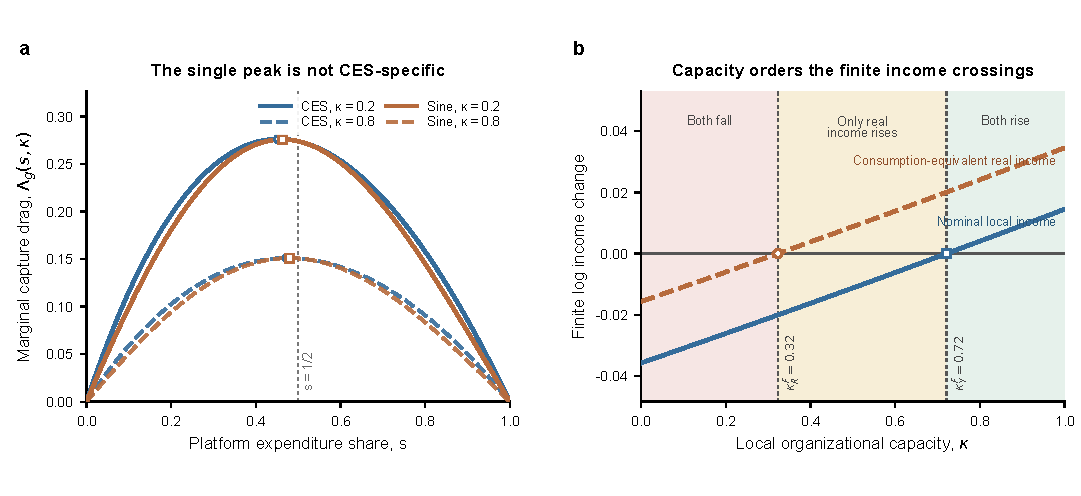
\includegraphics[width=\textwidth]{mechanism_figure.pdf}
 \caption{Capture drag and finite capacity thresholds. \textbf{(a)} CES
 \(g(s)=3s(1-s)\) and non-CES \(g(s)=0.75\sin(\pi s)\) are shown at
 \(\kappa=0.2\) and \(0.8\); both have a unique pre-half peak, and capacity
 moves it right while lowering it. \textbf{(b)} Finite log-income changes cross
 zero at \(\kappa_R^F=0.32<\kappa_Y^F=0.72\). Panel \textbf{(b)} uses the CES
 specialization with \(\alpha=0.35\), \(\beta=0.25\), \(a=0.4\), \(\eta=4\),
 \(\varepsilon=0.08\), \(\rho_A=0.8\),
 \((\underline\rho_P,\overline\rho_P)=(0.1,0.6)\), and
 \((z_0,z_1)=(-0.75,-0.30)\). Illustration, not calibration.}
 \label{fig:mechanisms}
\end{figure}

\section{Conclusion}
\label{sec:conclusion}

Market integration affects local income through access and the spatial
retention of transaction value. In the benchmark without outside-funded retail
spending, the endpoint-crossing condition yields ordered capacity thresholds
separating joint losses, consumption-equivalent real income gains with nominal
local-income losses, and joint gains. When platform transactions retain less
local income than local-agent transactions, the intermediate capture-drag peak
does not require CES: it follows from a strictly concave demand-induced
share-speed and precedes one-half under symmetry. In the same \(G=0\) benchmark,
a corollary establishes
increasing differences in both log-income measures. These results apply to a
short-run small-region closure with exogenous prices, capacity, and retention
schedules. The consumption-equivalent real-income index is not full welfare;
platform pricing, capacity investment, production relocation, and multi-region
feedback remain outside the model.

\section*{Data availability}

No data were used for the research described in this article.

\bibliographystyle{plainnat}
\bibliography{references}

\end{document}
